%!TEX root = ../main.tex

\chapter{Literature Review}\label{cha:literature}

Many extensive literature reviews and surveys have been written on the subject of deep learning.
In 1987, Lippmann reviewed 6 of the most influential Neural Networks of the era \cite{Lippmann_1987}.
More recently, an extensive Survey on Deep Learning in Medical Image Analysis was published \cite{Litjens_Kooi_Bejnordi_Setio_Ciompi_Ghafoorian_van_der_Laak_van_Ginneken_Sanchez_2017}.
In this, the use of deep learning for image classification, object detection and segmentation are all reviewed.
Also overviews of anatomical areas are provided, including neuro, retinal, pulmonary, digital pathology, breast, cardiac, abdominal and musculoskeletal.

\section{Deep Learning}\label{sec:deep_learning_lit}

\subsection{Training Deep Neural Networks}\label{subsec:training}
Due to the size of deep neural networks, and the non-convexity of the parameters, finding good optima has always been a challenge.
Stochastic gradient descent (SGD) has remained a popular strategy for researchers since the 80's although many optimisation algorithms are now used.
These include Adam \cite{Kingma_Ba_2014}, ADADELTA \cite{Zeiler_2012} and AdaGrad \cite{Duchi_Hazan_Singer_2011}.
For all of the optimisers mentioned, one of the main issues during training is choosing an appropriate learning rate.

It has been suggested by Dauphin et al. in \cite{Dauphin_de_Vries_Bengio_2015} that saddle points cause issues during training, not poor local optima.
However, in The Deep Learning Book \cite{Goodfellow-et-al-2016}, Goodfellow et al. prove that although learning is slow around saddle points due to the flatness, gradient based optimisation algorithms are still able to escape.

One possible solution is to use cyclical learning rates instead of a fixed learning rate that decreases over time.
A cycle has a fixed length and the learning rate varies between two sensible boundary values during that cycle.
This helps because if the optimisation gets stuck on a saddle plateau, increasing the learning rate will traverse the plateau quickly.

In Figure \ref{fig:triangular_cyclical_learning_rate} two methods for cyclical learning rates are shown.
Leslie N. Smith propesed these in \cite{Smith_2015}.
On the left plot min and max learning rate are kept the same, wheras on the right the difference is cut in half after each cycle.


\begin{figure}
    \centering
    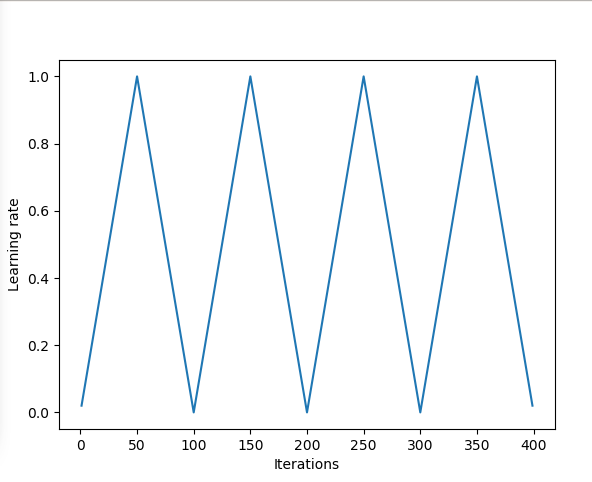
\includegraphics[width=0.45\textwidth]{./img/triangular.png}
    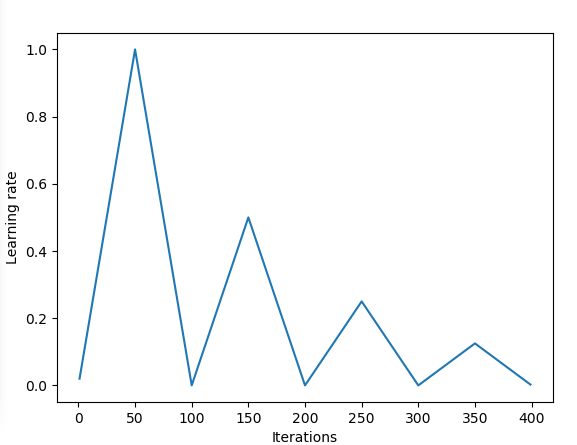
\includegraphics[width=0.45\textwidth]{./img/triangular2.png}
    \caption{Triangular and Triangular2 by Leslie N. Smith \cite{Smith_2015}.}
    \label{fig:triangular_cyclical_learning_rate}
\end{figure}

An alternative was suggest by Loshchilov and Hutter in \cite{Loshchilov_Hutter_2016}.
In this, the learning rate starts at its maximum and decreases to its minimum following the cosine function.
Once the minimum is reached the learning resets to the maximum, there is no increasing phase.
The authors also suggest making each cycle longer than the last by a constant factor they refer to as $T_{mult}$.

%TODO figures for cosine lr
\begin{figure}
    \centering
    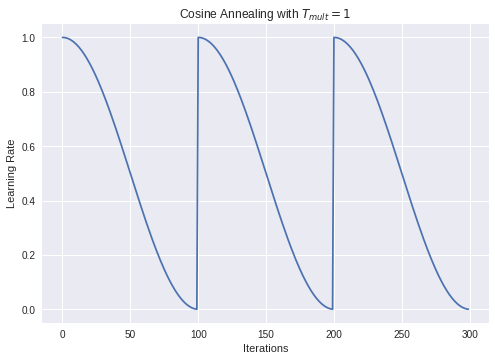
\includegraphics[width=0.45\textwidth]{./img/tmul1.png}
    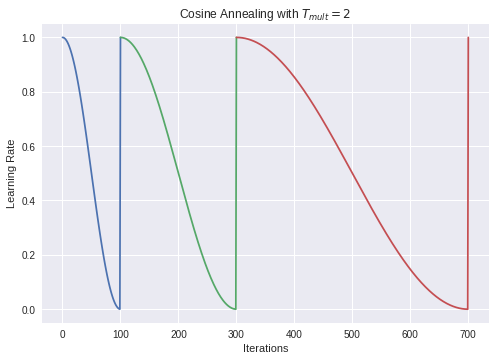
\includegraphics[width=0.45\textwidth]{./img/tmul2.png}
    \caption{Cosine Annealing with $T_{mult} = 1$ and $T_{mult} = 2$ by Loshchilov and Hutter \cite{Loshchilov_Hutter_2016}.}
    \label{fig:cosine_annealing}
\end{figure}

% TODO snapshot ensambling
People are well aware that ensemble methods produce great results.
Blah Blah outlined a method where models where saved periodically (Snapshot).
The period was large enough such that the models performed better/worse in different areas.
At prediction time they could be used as an ensemble. \cite{Huang_Li_Pleiss_Liu_Hopcroft_Weinberger_2017}

In \cite{Keskar_Mudigere_Nocedal_Smelyanskiy_Tang_2016} it is suggested that convergence to sharp minima leads to poor generalisation for deep learning.
Figure \ref{fig:wide_optima} outlines a sharp minimum.
Numerical evidence is then given that supports this view and several attempts to address the problem are presented.
However, initial results suggest that whilst these strategies do lead to better generalisation, they still converge to sharp minima.

\begin{figure}
    \centering
    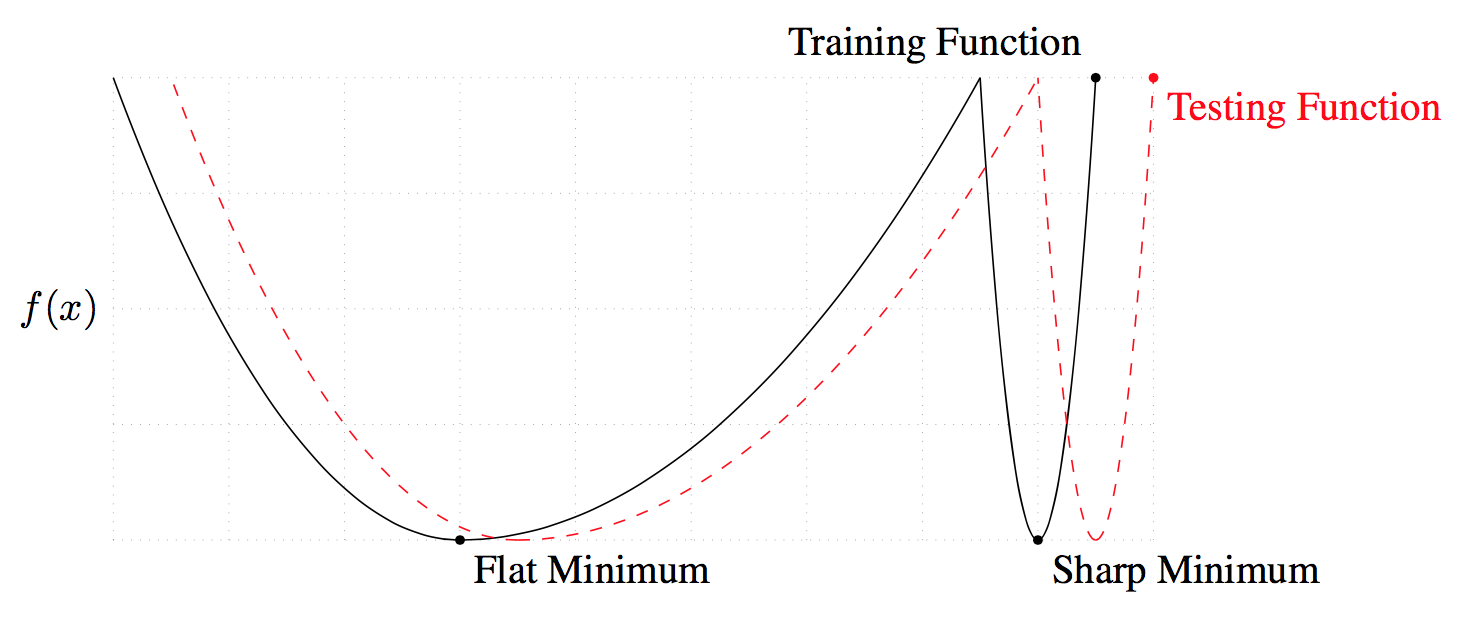
\includegraphics[width=\textwidth]{./img/Wide_optima.png}
    \caption{A Conceptual Sketch of Flat and Sharp Minima. The Y-axis indicates value of the loss function and the X-axis the variables (parameters) \cite{Keskar_Mudigere_Nocedal_Smelyanskiy_Tang_2016}}
    \label{fig:wide_optima}
\end{figure}


\subsection{Recent Developments}\label{subsec:recent_improvements}
% TODO Capsule
In late 2017, Hinton outlined a method for training capsule based methods.
This is something he'd been thinking about for years.
It learns pose representations of objects. \cite{Hinton_Sabour_Frosst_2018, Sabour_Frosst_Hinton_2017}



% TODO FGE
This is all taking an ensemble in model space, what if we do it in weight space.
(FGE) Someone else then showed that making the cycles short was still pretty good.
This is because because there exist connected paths of low loss between sufficiently different models, it is possible to travel along those paths in small steps and the models encountered along will be different enough to allow ensembling them with good results.
This is much faster
\cite{Garipov_Izmailov_Podoprikhin_Vetrov_Wilson_2018}



\begin{figure}
    \centering
    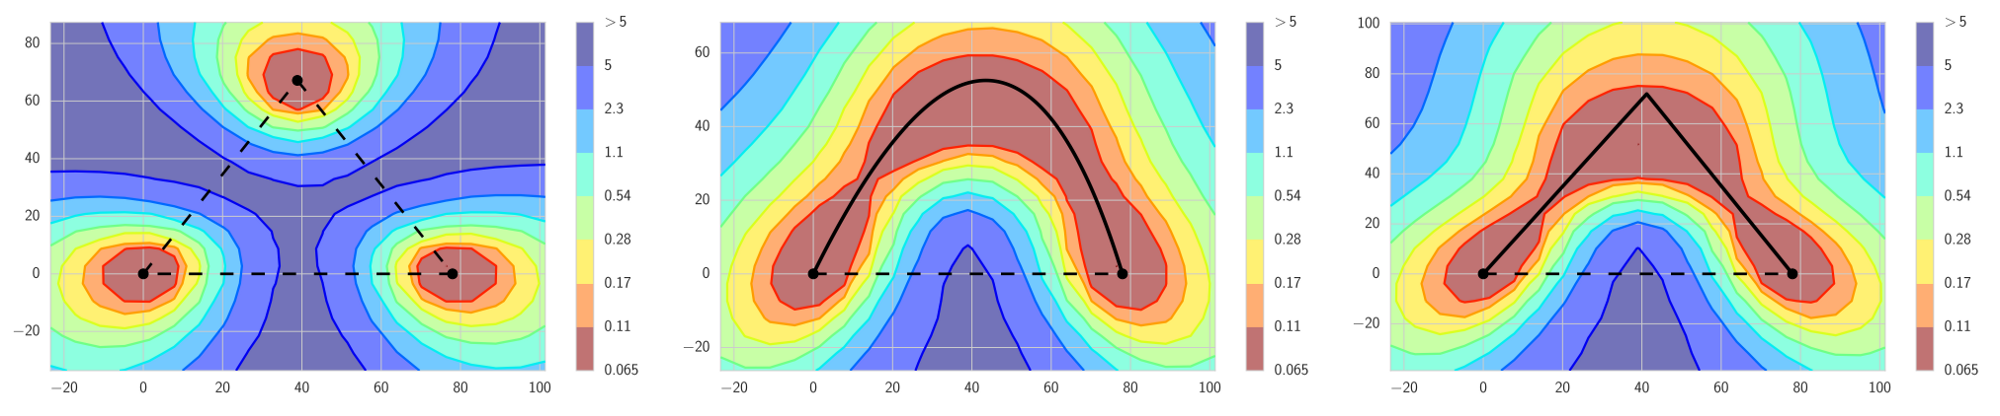
\includegraphics[width=\textwidth]{./img/FGE.png}
    \caption{}
    \label{fig:FGE_shortest_path}
\end{figure}

\begin{figure}
    \centering
    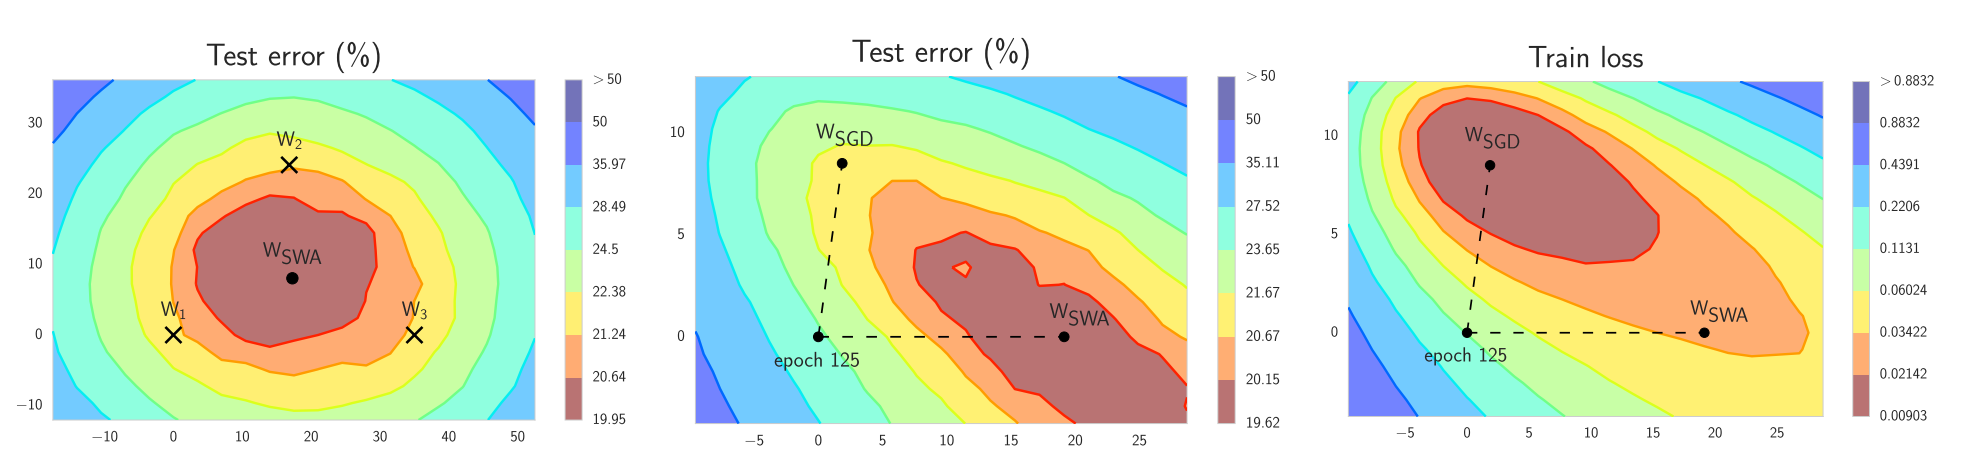
\includegraphics[width=\textwidth]{./img/SWA.png}
    \caption{\cite{Izmailov_Podoprikhin_Garipov_Vetrov_Wilson_2018}}
    \label{fig:SWA}
\end{figure}

% TODO SWA

We find that maintaining an average of the weights we encounter performs pretty well; it is better than snapshot and almost as good as FGE
This is much quicker and less computationally expensive because we don't have to carry around several different models. \cite{Izmailov_Podoprikhin_Garipov_Vetrov_Wilson_2018}

\section{Deep Learning in Medicine}\label{deep_learning_medic_lit}
% TODO section on deep learning in medicine
U-Net \cite{Ronneberger_Fischer_Brox_2015}
3D U Net \cite{Cicek_Abdulkadir_Lienkamp_Brox_Ronneberger_2016}

Cancer metastases \cite{Liu_Gadepalli_Norouzi_Dahl_Kohlberger_Boyko_Venugopalan_Timofeev_Nelson_Corrado_et_al_2017}

Dermatologist level skin cancer \cite{Esteva_Kuprel_Novoa_Ko_Swetter_Blau_Thrun_2017}

TernausNet (pretrained weights as encoder part of unet) \cite{Iglovikov_Shvets_2018}
